\documentclass{standalone}
\usepackage{tikz}
% all other packages and stuff you need for the picture
\usepackage{array}
\usepackage{pgfplots}
\usetikzlibrary{positioning}
\pgfplotsset{compat=1.18}

\begin{document}
		\begin{tabular}{|>{\centering\arraybackslash}m{6.5cm}|>{\centering\arraybackslash}m{6.5cm}|}
			\hline
			\multicolumn{2}{|c|}{\textbf{Porównanie funkcji i ich pochodnych}} \\
			\hline
			\textbf{Funkcja Heaviside $H(x)$} & \textbf{Pochodna $H(x)$} \\
			\hline
			% Wykresy: Heaviside i Dirac
			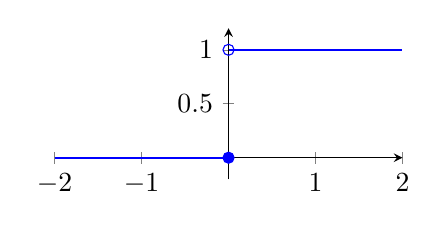
\begin{tikzpicture}[baseline=(current bounding box.center)]
				\begin{axis}[width=6cm, height=3.5cm,
					axis lines=middle, xmin=-2, xmax=2, ymin=-0.2, ymax=1.2]
					\addplot[blue, thick, domain=-2:0] {0};
					\addplot[blue, thick, domain=0:2] {1};
					\addplot[only marks, mark=*, blue] coordinates {(0,0)};
					\addplot[only marks, mark=o, blue] coordinates {(0,1)};
				\end{axis}
			\end{tikzpicture}
			&
			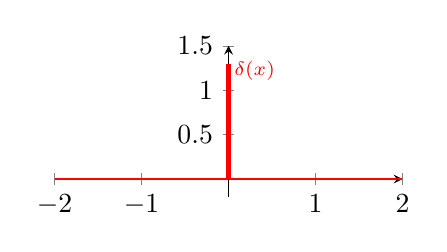
\begin{tikzpicture}[baseline=(current bounding box.center)]
				\begin{axis}[width=6cm, height=3.5cm,
					axis lines=middle, xmin=-2, xmax=2, ymin=-0.2, ymax=1.5]
					\addplot[red, thick, domain=-2:-0.01] {0};
					\addplot[red, thick, domain=0.01:2] {0};
					\addplot[red, ultra thick] coordinates {(0,0) (0,1.3)};
					\node[red, above] at (axis cs:0.3,1) {\scriptsize $\delta(x)$};
				\end{axis}
			\end{tikzpicture}
			\\
			\hline
			\textbf{Funkcja $ReLU(x)$} & \textbf{Pochodna $ReLU(x)$} \\
			\hline
			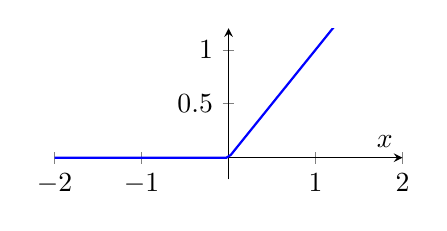
\begin{tikzpicture}
				\begin{axis}[
					axis lines=middle,
					xlabel={$x$},
					ylabel={},
					width=6cm,
					height=3.5cm,
					xmin=-2, xmax=2, ymin=-0.2, ymax=1.2,
					samples=200,
					domain=-5:5
					]
					% ReLU
					\addplot[blue, thick] {max(0,x)};
				\end{axis}
			\end{tikzpicture}
			&
			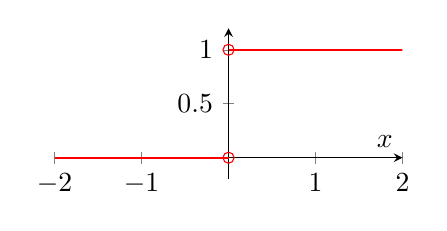
\begin{tikzpicture}
				\begin{axis}[
					axis lines=middle,
					xlabel={$x$},
					ylabel={},
					width=6cm,
					height=3.5cm,
					xmin=-2, xmax=2, ymin=-0.2, ymax=1.2,
					samples=200,
					domain=-5:5
					]
					% ReLU'
					% Lewa część (pochodna = 0)
					\addplot[red, thick, domain=-2:0] {0};
					% Prawa część (pochodna = 1)
					\addplot[red, thick, domain=0:2] {1};
					% Puste kółko w (0,0)
					\addplot[only marks, mark=o, mark size=2pt, color=red] coordinates {(0,0)};
					% Puste kółko w (0,1)
					\addplot[only marks, mark=o, mark size=2pt, color=red] coordinates {(0,1)};
				\end{axis}
			\end{tikzpicture}
			\\
			\hline
			\textbf{Tangens hiperboliczny $tanh(x)$} & \textbf{Pochodna $tanh(x)$} \\
			\hline
			% Możesz wstawić kolejne wykresy lub zostawić jako szablon:
			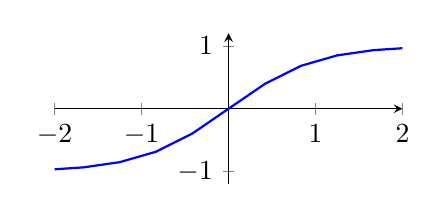
\begin{tikzpicture}
				\begin{axis}[width=6cm, height=3.5cm,
					axis lines=middle, xmin=-2, xmax=2, ymin=-1.2, ymax=1.2]
					% Wykres tanh(x)
					\addplot[blue, thick] {tanh(x)};
				\end{axis}
			\end{tikzpicture}
			& 
			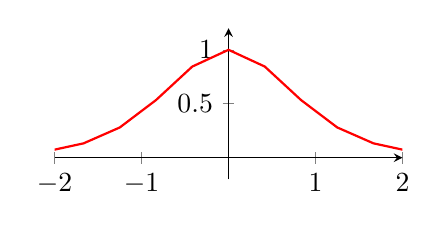
\begin{tikzpicture}
				\begin{axis}[width=6cm, height=3.5cm,
					axis lines=middle, xmin=-2, xmax=2, ymin=-0.2, ymax=1.2]
					% Pochodna: 1 - tanh^2(x)
					\addplot[red, thick] {1 - tanh(x)^2};
					
				\end{axis}
			\end{tikzpicture}
			\\
			\hline
			\textbf{ $\sigma(x)$} & \textbf{Pochodna $\sigma(x)$} \\
			\hline
			
			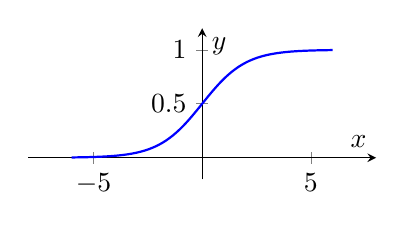
\begin{tikzpicture}
				\begin{axis}[
					width=6cm,
					height=3.5cm,
					axis lines=middle,
					xlabel={$x$},
					ylabel={$y$},
					xmin=-8, xmax=8,
					ymin=-0.2, ymax=1.2,
					samples=200,
					domain=-6:6
					]
					% Funkcja sigmoid
					\addplot[blue, thick] {1/(1+exp(-x))};
					
				\end{axis}
				
			\end{tikzpicture}
			&
			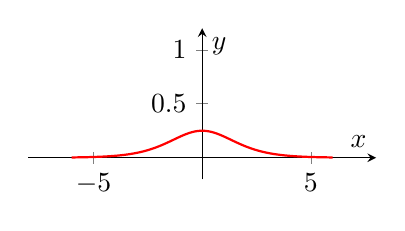
\begin{tikzpicture}
				\begin{axis}[
					width=6cm,
					height=3.5cm,
					axis lines=middle,
					xlabel={$x$},
					ylabel={$y$},
					xmin=-8, xmax=8,
					ymin=-0.2, ymax=1.2,
					samples=200,
					domain=-6:6
					]
					% Pochodna sigmoid
					\addplot[red, thick] 	{(1/(1+exp(-x)))*(1-1/(1+exp(-x)))};
				\end{axis}
			\end{tikzpicture}
			\\
			\hline
		\end{tabular}
\end{document}